% Options for packages loaded elsewhere
\PassOptionsToPackage{unicode}{hyperref}
\PassOptionsToPackage{hyphens}{url}
%
\documentclass[
]{article}
\usepackage{amsmath,amssymb}
\usepackage{lmodern}
\usepackage{ifxetex,ifluatex}
\ifnum 0\ifxetex 1\fi\ifluatex 1\fi=0 % if pdftex
  \usepackage[T1]{fontenc}
  \usepackage[utf8]{inputenc}
  \usepackage{textcomp} % provide euro and other symbols
\else % if luatex or xetex
  \usepackage{unicode-math}
  \defaultfontfeatures{Scale=MatchLowercase}
  \defaultfontfeatures[\rmfamily]{Ligatures=TeX,Scale=1}
\fi
% Use upquote if available, for straight quotes in verbatim environments
\IfFileExists{upquote.sty}{\usepackage{upquote}}{}
\IfFileExists{microtype.sty}{% use microtype if available
  \usepackage[]{microtype}
  \UseMicrotypeSet[protrusion]{basicmath} % disable protrusion for tt fonts
}{}
\makeatletter
\@ifundefined{KOMAClassName}{% if non-KOMA class
  \IfFileExists{parskip.sty}{%
    \usepackage{parskip}
  }{% else
    \setlength{\parindent}{0pt}
    \setlength{\parskip}{6pt plus 2pt minus 1pt}}
}{% if KOMA class
  \KOMAoptions{parskip=half}}
\makeatother
\usepackage{xcolor}
\IfFileExists{xurl.sty}{\usepackage{xurl}}{} % add URL line breaks if available
\IfFileExists{bookmark.sty}{\usepackage{bookmark}}{\usepackage{hyperref}}
\hypersetup{
  pdftitle={High Dimensional Data Analysis - Group Assignment 18},
  pdfauthor={Dewi Amaliah, Aarathy Babu, Rahul Bharadwaj \& Priya Dingorkar},
  hidelinks,
  pdfcreator={LaTeX via pandoc}}
\urlstyle{same} % disable monospaced font for URLs
\usepackage[margin=1in]{geometry}
\usepackage{longtable,booktabs,array}
\usepackage{calc} % for calculating minipage widths
% Correct order of tables after \paragraph or \subparagraph
\usepackage{etoolbox}
\makeatletter
\patchcmd\longtable{\par}{\if@noskipsec\mbox{}\fi\par}{}{}
\makeatother
% Allow footnotes in longtable head/foot
\IfFileExists{footnotehyper.sty}{\usepackage{footnotehyper}}{\usepackage{footnote}}
\makesavenoteenv{longtable}
\usepackage{graphicx}
\makeatletter
\def\maxwidth{\ifdim\Gin@nat@width>\linewidth\linewidth\else\Gin@nat@width\fi}
\def\maxheight{\ifdim\Gin@nat@height>\textheight\textheight\else\Gin@nat@height\fi}
\makeatother
% Scale images if necessary, so that they will not overflow the page
% margins by default, and it is still possible to overwrite the defaults
% using explicit options in \includegraphics[width, height, ...]{}
\setkeys{Gin}{width=\maxwidth,height=\maxheight,keepaspectratio}
% Set default figure placement to htbp
\makeatletter
\def\fps@figure{htbp}
\makeatother
\setlength{\emergencystretch}{3em} % prevent overfull lines
\providecommand{\tightlist}{%
  \setlength{\itemsep}{0pt}\setlength{\parskip}{0pt}}
\setcounter{secnumdepth}{-\maxdimen} % remove section numbering
\usepackage{booktabs}
\usepackage{longtable}
\usepackage{array}
\usepackage{multirow}
\usepackage{wrapfig}
\usepackage{float}
\usepackage{colortbl}
\usepackage{pdflscape}
\usepackage{tabu}
\usepackage{threeparttable}
\usepackage{threeparttablex}
\usepackage[normalem]{ulem}
\usepackage{makecell}
\usepackage{xcolor}
\ifluatex
  \usepackage{selnolig}  % disable illegal ligatures
\fi

\title{\textbf{High Dimensional Data Analysis - Group Assignment 18}}
\author{\textbf{Dewi Amaliah, Aarathy Babu, Rahul Bharadwaj \& Priya Dingorkar}}
\date{9th September 2021}

\begin{document}
\maketitle

{
\setcounter{tocdepth}{1}
\tableofcontents
}
\pagebreak

\hypertarget{introduction}{%
\section{Introduction}\label{introduction}}

The UCLA-LoPucki Bankruptcy Research Database (BRD) is a UCLA School of Law data gathering, data linking, and data distribution initiative. The goal of the BRD is to encourage bankruptcy research by making bankruptcy data available to academic investigators worldwide. All of the data was gathered when the companies declared bankruptcy. In this study, we will use a variety of high-dimensional analysis approaches like Multidimesnionla Scaling, Principle Component Analysis and Clustering to extract useful insights from the data.

\begin{center}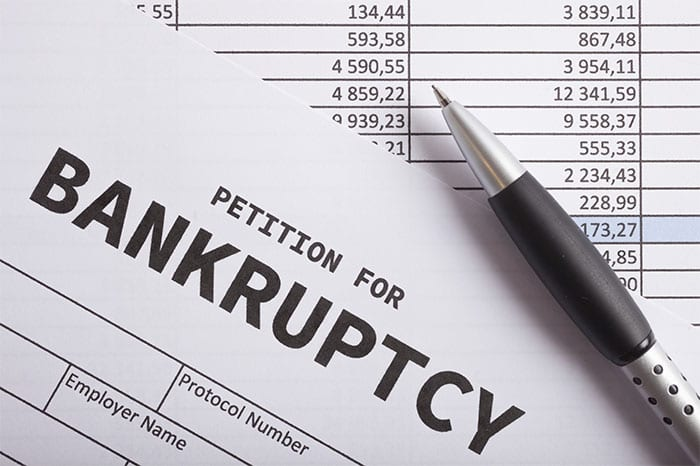
\includegraphics[width=450px]{data/bank} \end{center}

\pagebreak

\hypertarget{acknowledgement}{%
\section{Acknowledgement}\label{acknowledgement}}

Our sincere gratitude goes out to Ruben Loaiza-Maya and the our tutor Ari Handayani for their guidance and support. Our heartfelt thanks go to Ruben Loaiza-Maya and our instructor Ari Handayani for their advice and assistance. Their culminating efforts have placed us in a situation where we can produce this report collectively while showcasing our competence to employ diverse solutions that can be used with high dimensional data.

\pagebreak

\hypertarget{data-description}{%
\section{Data Description}\label{data-description}}

This report is based on data from US businesses that declared bankruptcy between 1980 and 2000. The information is coming from the UCLA-LoPucki Brankruptcy Research Database. Let's take a closer look at these variables and what they mean. Let's go further into the dataset to see if we can find any examples of data cleaning or wrangling.

The dataset has 436 observations and 7 variables with their description explained below.

\begin{itemize}
\tightlist
\item
  Name: Name of the firm
\item
  Assets: Total assets (in millions of dollars)
\item
  CityFiled: City where filing took place
\item
  CPI U.S CPI at the time of filing
\item
  DaysIn: Length of bankruptcy process
\item
  DENYOther: CityFiled, categorized as Wilmington (DE), New York (NY) or all other cities (OT)
\item
  Ebit: Earnings (operating income) at time of filing (in millions of dollars)
\item
  Employees: Number of employees before bankruptcy
\item
  EmplUnion: Number of union employees before bankruptcy
\item
  FilingRate: Total number of other bankrupcy filings in the year of this filing
\item
  FirmEnd: Short description of the event that ended the firm's existence
\item
  GDP: Gross Domestic Product for the Quarter in which the case was filed
\item
  HeadCityPop: The population of the firms headquarters city
\item
  HeadCourtCityToDE: The distance in miles from the firms headquarters city to the city in which
  the case was filed
\item
  HeadStAtFiling: The state in which firms headquarters is located
\item
  Liab: Total amount of money owed (in millions of dollars)
\item
  MonthFiled: Categorical variable where numbers from 1 to 12 correspond to months from Jan to Dec
\item
  PrimeFiling: Prime rate of interest on the bankruptcy filing date
\item
  Sales: Sales before bankruptcy (in dollars)
\item
  SICMajGroup: Standard industrial clasification code
\item
  YearFiled: Year bankruptcy was filed
\end{itemize}

Let us further examine the bankruptcy statistics. We will undertake some data analysis exploratory stages as well as data analysis, data cleansing and discussion. We will also go through the numerous approaches used for this high-dimensional data in detail later. The clean dataset is then submitted to multidimensional scales, analysis of principal components and clustering and to find about what the bankruptcy data would be most actionable. We will also examine the limitations and conclusions of our investigation.

\pagebreak

\hypertarget{princple-component-analysis-pca}{%
\section{Princple Component Analysis (PCA)}\label{princple-component-analysis-pca}}

Now that we've seen how to input this high-dimensional data into Multidimensional scaling (MDS) to obtain a low (typically 2) dimensional representation. Let us now perform a Principal Component Analysis (PCA), which is a dimensional-reduction method that is frequently used to reduce the dimensional of large data sets by transforming a large set of variables into a smaller one that still contains the majority of the information in the large set.

\begin{itemize}
\item
  Let's carry out PCA on our bankruptcy data. Lets investigate if our data is a good fit for PCA. Let's us further investigate how the variables in our data are correlated and many PC's explain the variation of our data.
\item
  Before we apply the this principle to our data, it is very important we standardized our variables as this ensures that results are not sensitive to the units of measurement. Thus giving us more accurate analysis.
\end{itemize}

\begin{verbatim}
## Importance of components:
##                          PC1    PC2    PC3     PC4    PC5     PC6     PC7
## Standard deviation     1.900 1.6842 1.1354 1.02794 0.9392 0.85634 0.82987
## Proportion of Variance 0.301 0.2364 0.1074 0.08806 0.0735 0.06111 0.05739
## Cumulative Proportion  0.301 0.5374 0.6448 0.73283 0.8063 0.86745 0.92484
##                            PC8     PC9    PC10    PC11   PC12
## Standard deviation     0.68629 0.49184 0.39448 0.14244 0.1148
## Proportion of Variance 0.03925 0.02016 0.01297 0.00169 0.0011
## Cumulative Proportion  0.96409 0.98424 0.99721 0.99890 1.0000
\end{verbatim}

\begin{itemize}
\tightlist
\item
  Using the \texttt{summary} function we can infer the following:

  \begin{itemize}
  \tightlist
  \item
    Proportion of variance explained by the first four PCs together is 73.28\%
  \item
    Proportion of variance explained by the first and second PC alone is 30.10\% and 23.64\% respectively
  \item
    Using kaisers rule, choose those PC's whose variance and standard deviation greater than 1, in our bankruptcy data we will choose 4 PC's.
  \end{itemize}
\item
  Let us now plot use the scree plot to find the total number of PC's that best explain our data.
\end{itemize}

\begin{center}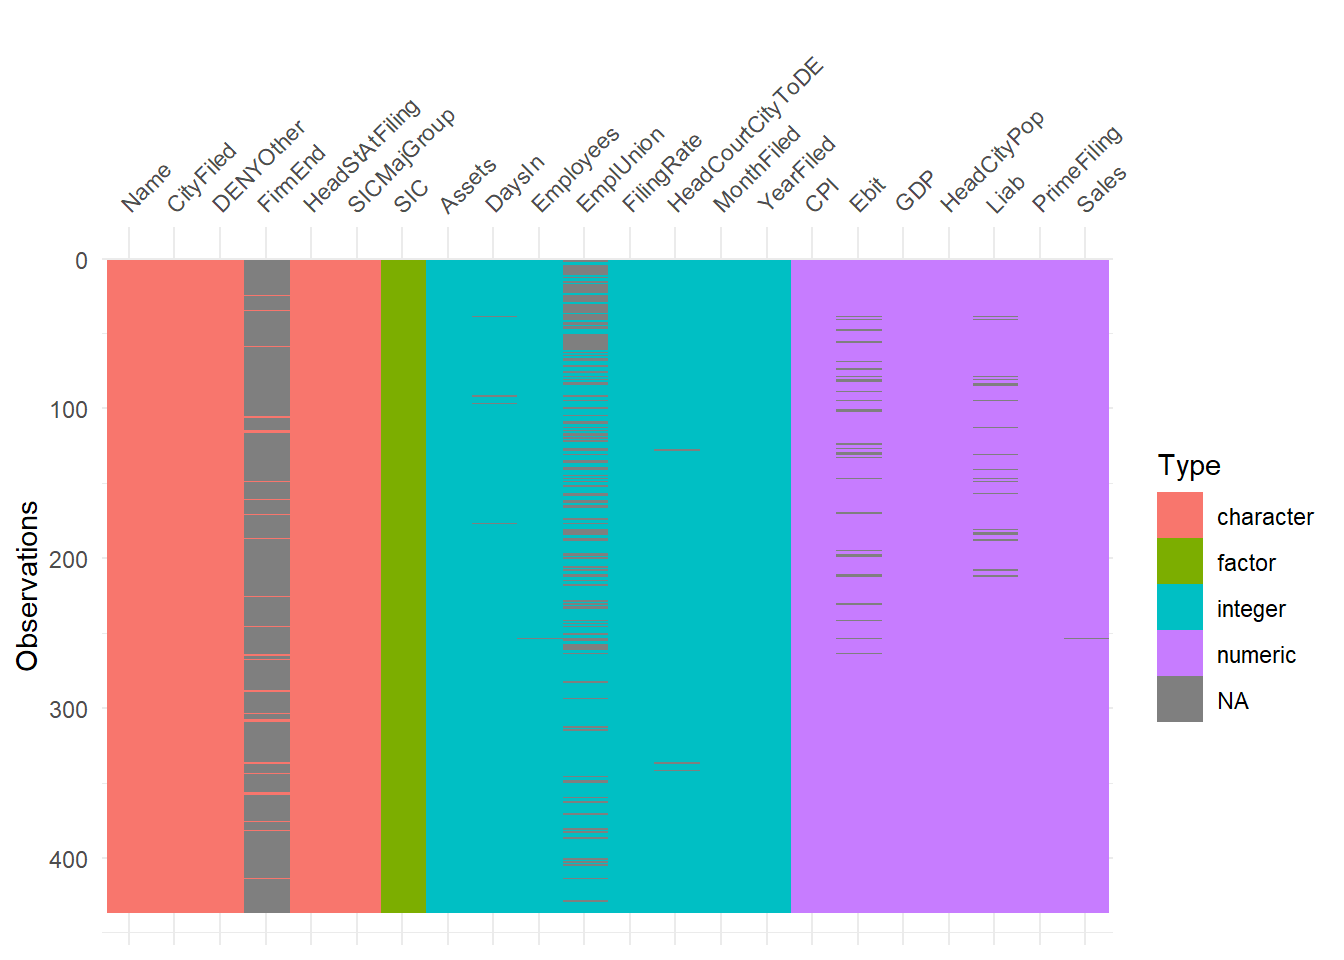
\includegraphics{report_files/figure-latex/unnamed-chunk-5-1} \end{center}

\begin{itemize}
\item
  Using the scree plot we infer that our bankruptcy data is explained by the first three PC's. Also note this is different to kaisers rule.
\item
  Let us now plot a biplot, that will help us infer intersting features about our data. A PCA biplot shows both PC scores of samples (dots) and loadings of variables(vectors).
\end{itemize}

\textbackslash begin\{figure\}

\{\centering \includegraphics{report_files/figure-latex/biplot_bank-1}

\}

\caption{PCA Biplot}

(\#fig:biplot\_bank)
\textbackslash end\{figure\}

\begin{itemize}
\item
  Looking at figure @ref(fig:biplot\_bank), more closely we infer that there is one company that is an outlier to our analysis. PCA allows us to infer that since this observation is very far apart from our variables direction it is best to remove this observation from our data and fit PCA again.
\item
  On further examination on this outlier we infer that Texaco Inc.~which comes under Petroleum SIC and Refining And Related Industries is the outlier in our bankruptcy data. This also agrees with our MDS method where we saw the same observations. Let us omit this observation and fit our PCA again.
\end{itemize}

\end{document}
